\documentclass[12pt,a4paper]{article}

% --- Page Geometry & Margins ---
\usepackage[margin=1in]{geometry}
\usepackage{parskip}          % Modern block paragraph spacing
\usepackage{tabularx}
\usepackage{float}
\usepackage{tikz}
\usetikzlibrary{shapes.geometric, arrows.meta, positioning, fit, backgrounds}
% --- Typography & Readability ---
\usepackage[utf8]{inputenc}
\usepackage[T1]{fontenc}
\usepackage{lmodern}
\usepackage{setspace}
\onehalfspacing
\usepackage{microtype}

% --- Headers & Footers ---
\usepackage{fancyhdr}
\pagestyle{fancy}
\fancyhf{}
\lhead{\small\textbf{Prototype Stage Report}}
\rhead{\small WASM Port of GTA III}
\cfoot{\small \thepage}
\renewcommand{\headrulewidth}{0.4pt}
\renewcommand{\footrulewidth}{0pt}

% --- Section Styling ---
\usepackage{titlesec}
\titleformat{\section}
  {\normalfont\Large\bfseries}{\thesection}{1em}{}[\titlerule]
\titlespacing*{\section}{0pt}{2.5ex plus 1ex minus .2ex}{1.2ex plus .2ex}

% --- Highlight Callout Box (Monochrome) ---
\usepackage[many]{tcolorbox}
\newtcolorbox{summarybox}[1][]{
  colback=white,
  colframe=black,
  arc=2pt,
  boxrule=0.8pt,
  left=10pt, right=10pt, top=8pt, bottom=8pt,
  fonttitle=\bfseries,
  #1
}

% --- Tables & Figures ---
\usepackage{booktabs}
\usepackage{graphicx}
\usepackage{caption}
\captionsetup{labelfont=bf, textfont=it, margin=10pt}

% --- Math & Hyperlinks (All Black) ---
\usepackage{amsmath, amssymb}
\usepackage{hyperref}
\hypersetup{
    hidelinks,
    pdfauthor={Antriksh, Divyam Jain},
    pdftitle={WASM Port of Grand Theft Auto 3 - Prototype Report},
    pdfpagemode=UseOutlines
}

% =========================================================================
% DOCUMENT BEGINS
% =========================================================================
\begin{document}

% --- Cover Page ---
\begin{titlepage}
    \centering
    \vspace*{1.5cm}
    
    {\Huge \textbf{Project Prototype Report}} \\[0.5cm]
    {\Large \textbf{WebAssembly Port of Grand Theft Auto III}} \\
    
    \vspace{1.5cm}
    \rule{\linewidth}{1pt} \\
    \vspace{1.5cm}
    
    \begin{minipage}{0.48\textwidth}
        \begin{flushleft} \large
            \textbf{Prepared By:}\\
            Antriksh (1024031032)\\
            Divyam Jain (1024031032)
        \end{flushleft}
    \end{minipage}
    \begin{minipage}{0.48\textwidth}
        \begin{flushright} \large
            \textbf{Supervised By:}\\
            Professor Nisha Thakur
        \end{flushright}
    \end{minipage}

    \vfill

    {\large \textbf{Date:} \today}
\end{titlepage}

% --- Abstract ---
\begin{abstract}
\noindent This report details the prototype implementation of porting Grand Theft Auto III to the web browser utilizing WebAssembly (WASM), WebGL 2.0, and the Emscripten toolchain based on the open-source reverse-engineered engine codebase (\texttt{re3}). The project aims to eliminate the need for native platform binaries or external installations by executing legacy C++ game engines natively inside modern web browsers. This prototype demonstrates successful compilation of core C++ engine components, basic WebGL graphics context initialization, asynchronous asset fetching over HTTP, and frame-rate synchronization within browser execution contexts.
\end{abstract}

\newpage

% --- Table of Contents ---
\tableofcontents
\thispagestyle{plain}
\newpage

% --- Main Body ---
\section{Introduction \& Objectives}

\subsection{Project Background}
Historically, AAA desktop games like Grand Theft Auto III relied on native platform architectures (x86/Win32) tied directly to native graphics APIs like DirectX 8/9. Bringing complex legacy C++ codebases to modern browsers requires bypassing traditional platform dependencies. WebAssembly (WASM) provides a low-level, high-performance bytecode format capable of running C/C++ code in client-side browser sandboxes at near-native speed. By leveraging the open-source reverse-engineered GTA III codebase (\texttt{re3}), this project translates standard RenderWare graphics calls and platform abstraction layers into browser-compatible web primitives.

\subsection{Prototype Objectives}
The scope of this prototype evaluation encompasses the following milestones:
\begin{itemize}
    \item Cross-compiling the \texttt{re3} C++ source code to \texttt{.wasm} binaries via the Emscripten toolchain.
    \item Mapping native RenderWare/OpenGL calls to a WebGL 2.0 browser pipeline.
    \item Replacing desktop event handling (Win32 API/DirectInput) with browser event listeners and SDL2 input wrappers.
    \item Evaluating memory management constraints within the browser's 32-bit WASM Linear Memory address space.
\end{itemize}

\begin{summarybox}[title=Prototype Target State]
Achieve a playable main menu and stable rendering of initial indoor and outdoor game scenes directly inside Chrome and Firefox without external plugins.
\end{summarybox}

\section{System Architecture \& Design}

\subsection{System Overview}
The system architecture bridges the compiled native game logic with standard web platform APIs. Emscripten acts as the intermediary compiler layer, generating a JavaScript runtime bridge that hooks browser user inputs, GPU draws, and file system interactions directly into the compiled WebAssembly heap.

\begin{figure}[H]
\centering
\resizebox{\textwidth}{!}{%
\begin{tikzpicture}[
    actor/.style={rectangle, draw=black, thick, fill=gray!20, rounded corners=3pt, minimum height=2.5em, text width=6.5em, align=center, font=\small\bfseries},
    usecase/.style={ellipse, draw=black, thick, fill=white, minimum height=2.4em, text width=10em, align=center, font=\small},
    boundary/.style={rectangle, draw=black!80, thick, dashed, fill=gray!5, inner sep=18pt, rounded corners=6pt},
    line/.style={draw=black, thick}
]

    % --- Actors ---
    \node [actor] (player) {End User / Player};
    \node [actor, right=11cm of player] (browser) {Browser Engine (Chrome/Firefox)};

    % --- System Boundary & Use Cases ---
    \node [usecase, right=2.5cm of player, yshift=3.5cm] (uc1) {Bootstrap WASM Module};
    \node [usecase, below=0.6cm of uc1] (uc2) {Mount Assets to MEMFS / IndexedDB};
    \node [usecase, below=0.6cm of uc2] (uc3) {Execute C++ Game Engine Logic};
    \node [usecase, below=0.6cm of uc3] (uc4) {Render 3D Frames via WebGL 2.0};
    \node [usecase, below=0.6cm of uc4] (uc5) {Process WebAudio Streams};
    \node [usecase, below=0.6cm of uc5] (uc6) {Capture HTML5 Mouse/Keyboard Inputs};

    % System Boundary Box
    \begin{scope}[on background layer]
        \node [boundary, fit=(uc1) (uc6), label={[font=\small\bfseries\color{black!80}]above:WASM GTA III Engine Boundary}] (system_box) {};
    \end{scope}

    % --- Connections ---
    % Player interactions
    \path [line] (player) -- (uc1);
    \path [line] (player) -- (uc6);

    % Browser interactions
    \path [line] (browser) -- (uc1);
    \path [line] (browser) -- (uc2);
    \path [line] (browser) -- (uc4);
    \path [line] (browser) -- (uc5);

    % Engine internal relationships
    \path [line, dashed] (uc1) -- node[left, font=\tiny]{«include»} (uc2);
    \path [line, dashed] (uc2) -- node[left, font=\tiny]{«include»} (uc3);
    \path [line, dashed] (uc3) -- node[left, font=\tiny]{«include»} (uc4);
    \path [line, dashed] (uc3) -- node[left, font=\tiny]{«include»} (uc5);

\end{tikzpicture}
}
\caption{Use Case Diagram illustrating system actors, engine boundaries, and web platform integration.}
\label{fig:use_case}
\end{figure}

\subsection{Data Flow Analysis}
The data flow within the WebAssembly execution model maps standard desktop system interactions into asynchronous browser streams. Figure~\ref{fig:dfd0} and Figure~\ref{fig:dfd1} illustrate the high-level context DFD and detailed subsystem data transformations across the virtual filesystem and WebGL render loop.

\begin{figure}[H]
    \centering
    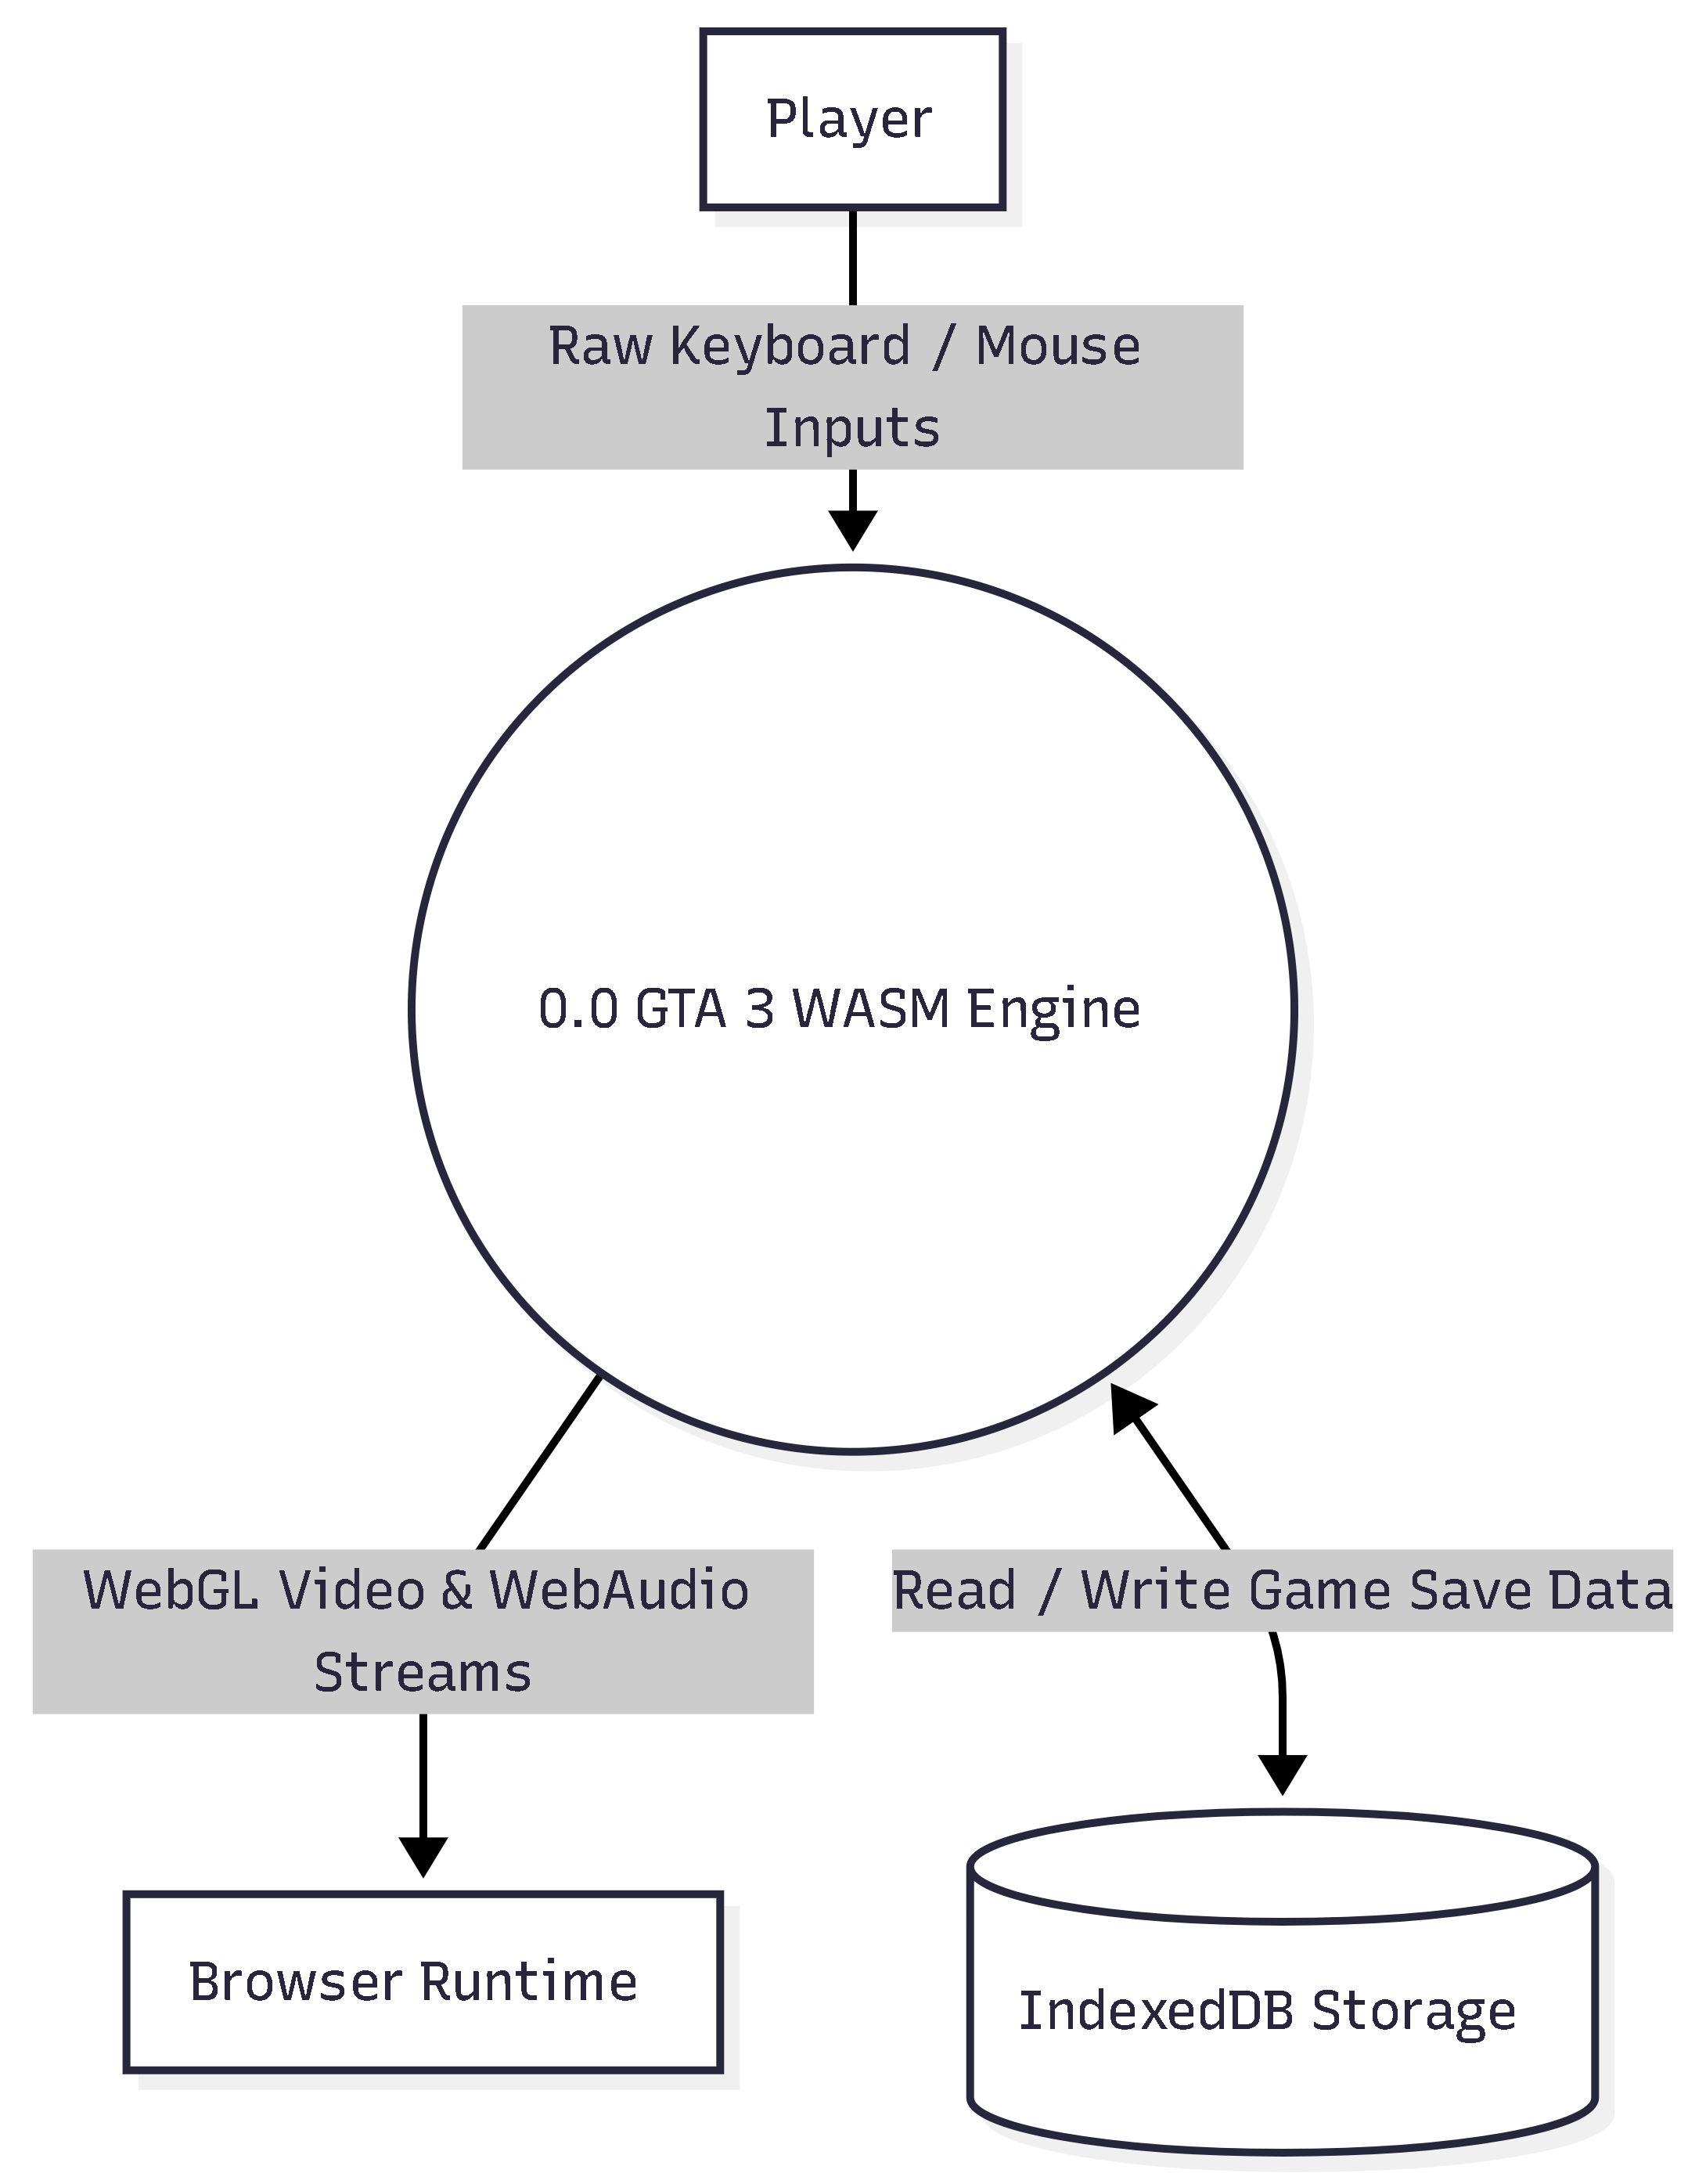
\includegraphics[width=0.8\textwidth]{dfd_level_0.png}
    \caption{Context-Level Data Flow Diagram (DFD Level 0).}
    \label{fig:dfd0}
\end{figure}

\begin{figure}[H]
    \centering
    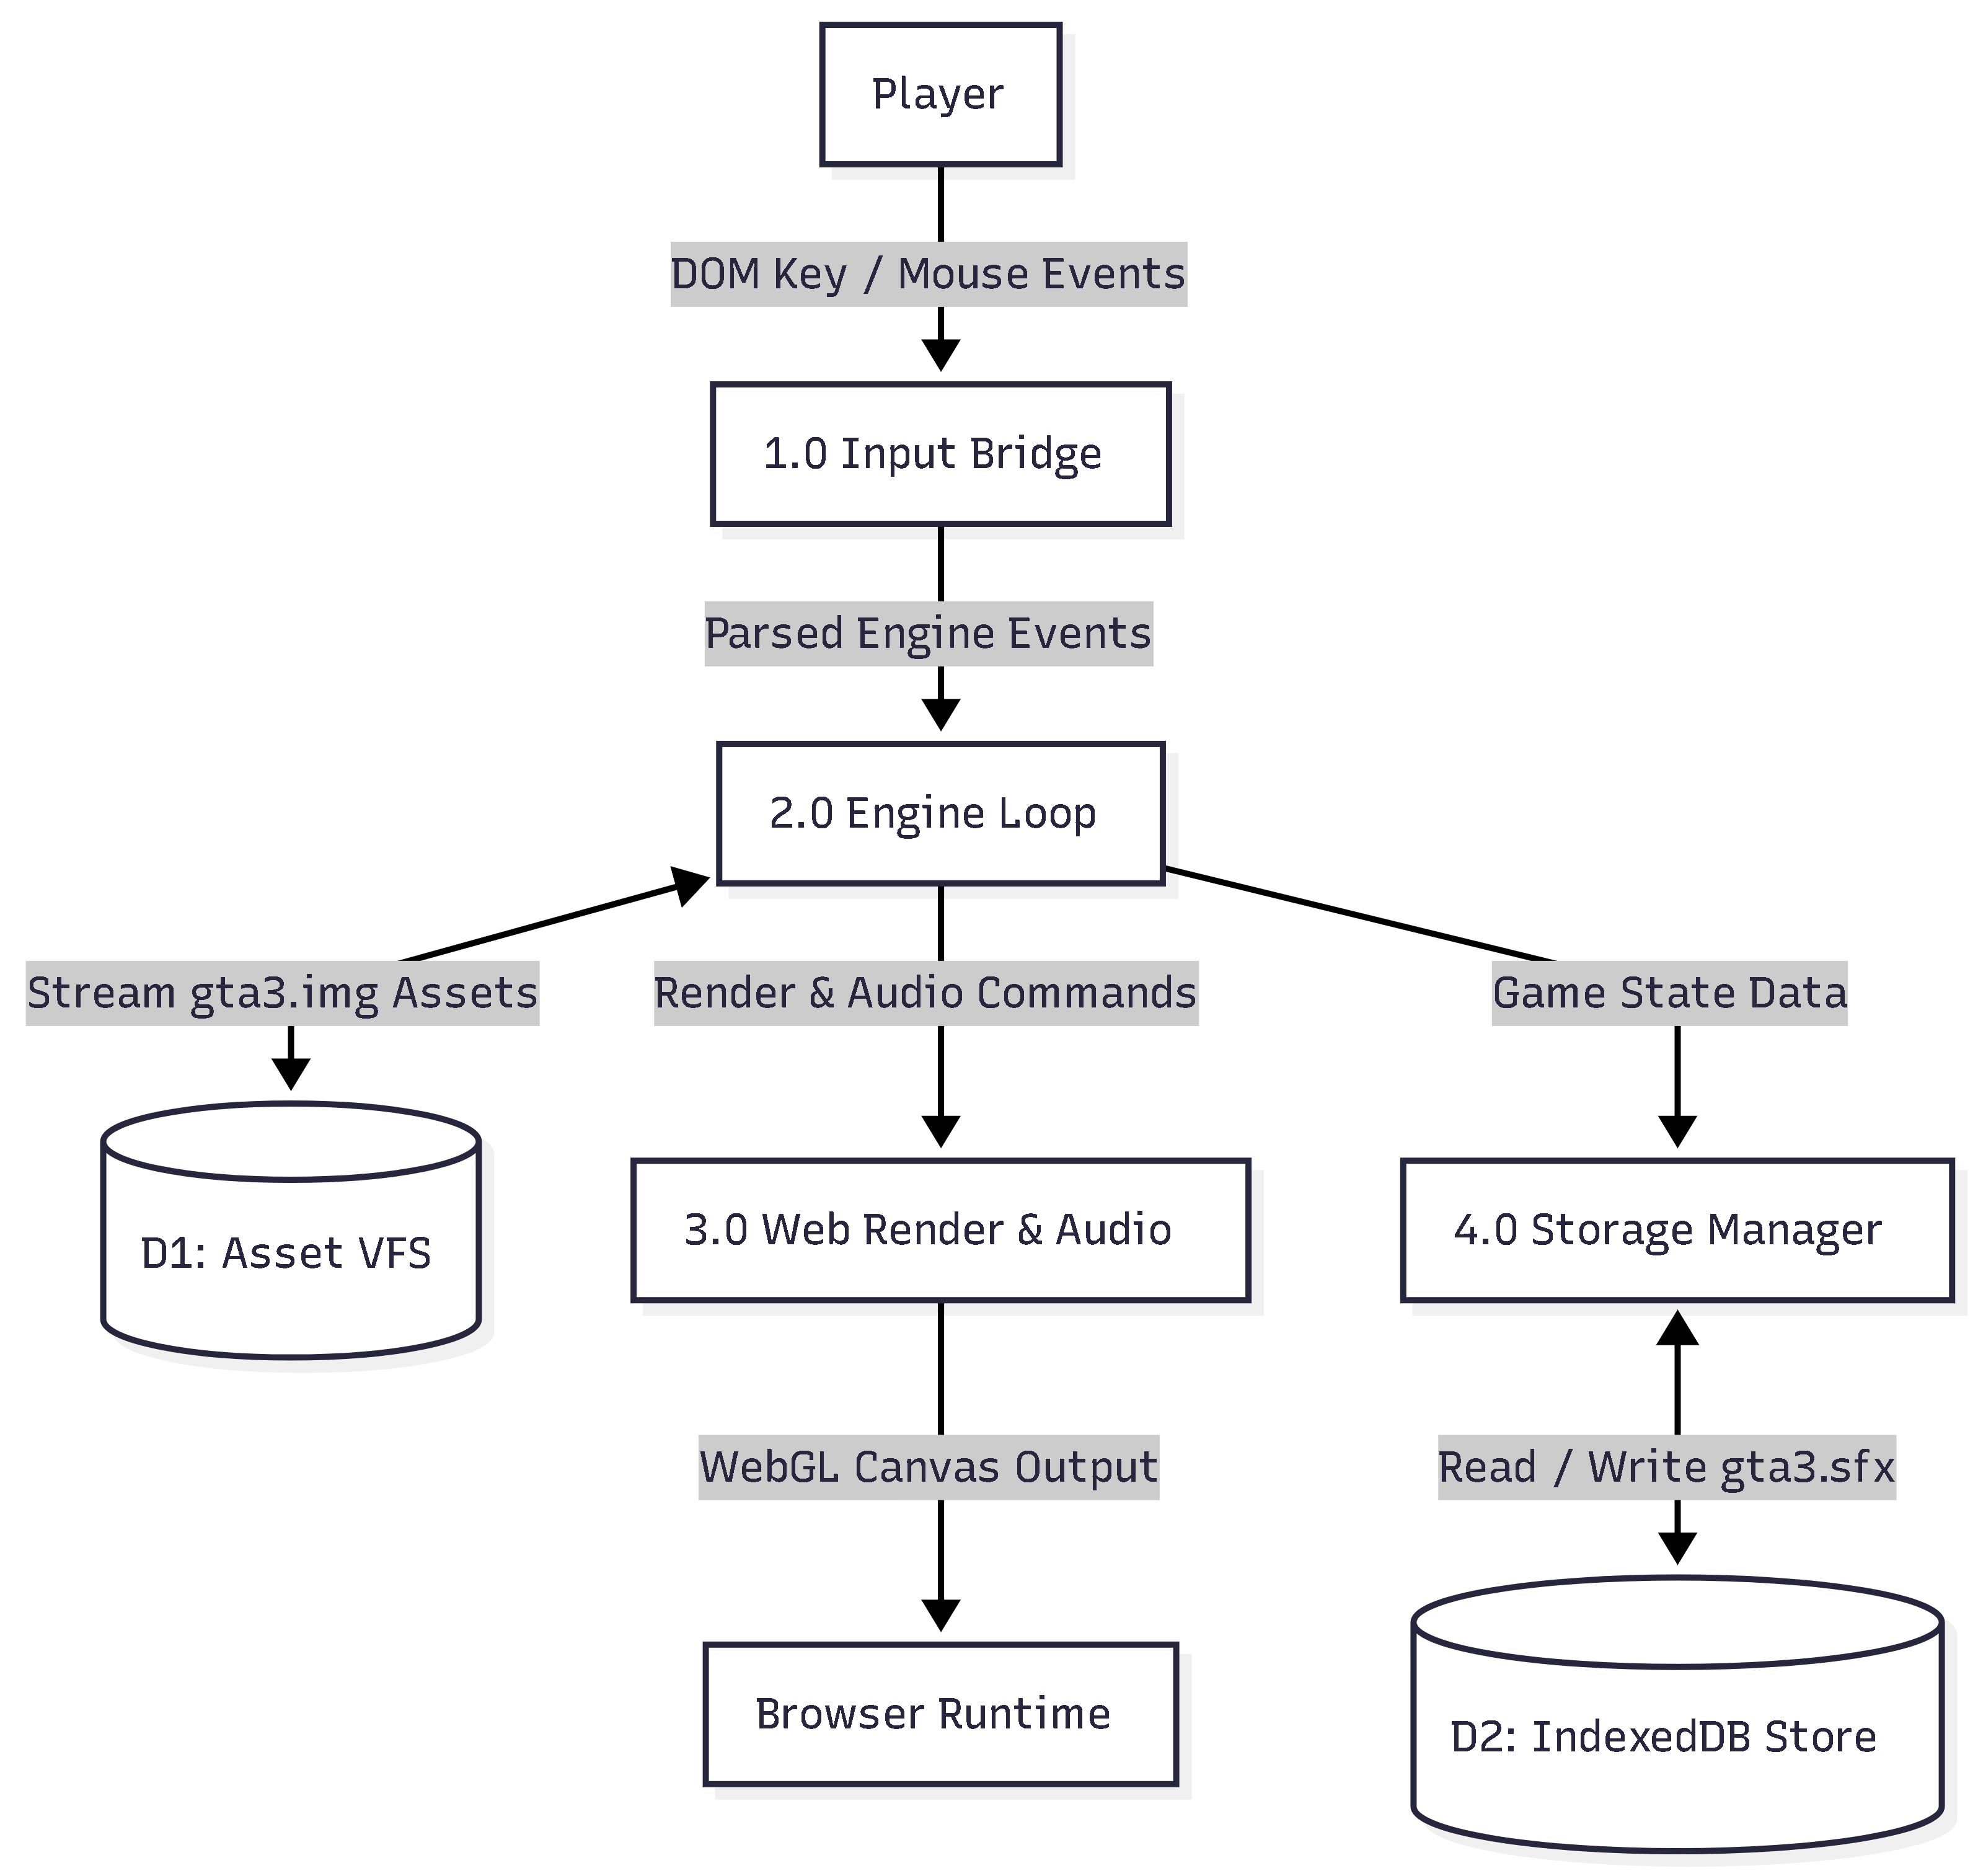
\includegraphics[width=0.85\textwidth]{dfd_level_1.png}
    \caption{Subsystem Data Flow Diagram (DFD Level 1).}
    \label{fig:dfd1}
\end{figure}

\subsection{Component Specifications}
The system architecture consists of several modular subsystems designed to translate desktop dependencies into native browser standards. Table~\ref{tab:specifications} outlines the specific technology stack components and their core operational roles within the WebAssembly execution environment.

\begin{table}[H]
\centering
\caption{System Layer Architecture \& Toolchain Setup}
\label{tab:specifications}
\begin{tabularx}{\textwidth}{l l X}
\toprule
\textbf{Layer} & \textbf{Technology Stack} & \textbf{Function / Responsibility} \\
\midrule
Source Engine      & C++ / \texttt{re3} Codebase      & Core game state logic and entity handling \\
Compilation        & Emscripten (LLVM/Clang)  & Translates C++ AST to WebAssembly bytecode \\
Graphics Pipeline  & WebGL 2.0 / OpenGL ES 3.0 & Renders game geometry, meshes, and textures \\
Audio Pipeline     & WebAudio API / OpenAL    & Handles 3D positional audio streaming \\
Asset System       & Emscripten Virtual FS    & Virtualizes game archive files (\texttt{.img}/\texttt{.dir}) \\
Input System       & HTML5 Events / SDL2      & Captures mouse movement and keyboard states \\
\bottomrule
\end{tabularx}
\end{table}
\section{Prototype Implementation}

\subsection{Build Toolchain \& WebAssembly Compilation}
The cross-compilation pipeline utilizes Emscripten to transform native C++ routines into optimized WASM bytecode. The main rendering loop is adapted to prevent thread-blocking within the browser's main thread by replacing execution loops with non-blocking browser animation frame callbacks:

$$\text{Engine Execution Loop} \longrightarrow \texttt{emscripten\_set\_main\_loop(GameLoop, 0, 1)}$$

Standard POSIX file operations are bound to Emscripten's MEMFS virtual filesystem, enabling the C++ engine to read game textures, models, and scripts as if accessing a local hard drive.

\subsection{Runtime Memory \& Graphics Mapping}
\begin{itemize}
    \item \textbf{WASM Memory Heap:} A contiguous 512 MB block of WebAssembly Linear Memory is pre-allocated to accommodate game state variables, dynamic entity pools, and texture buffers.
    \item \textbf{RenderWare Integration:} RenderWare's native backend functions are translated into OpenGL ES commands, which Emscripten routes directly to WebGL 2.0 contexts embedded inside an HTML5 Canvas element.
\end{itemize}
\begin{figure}[H]
\centering
\resizebox{\textwidth}{!}{%
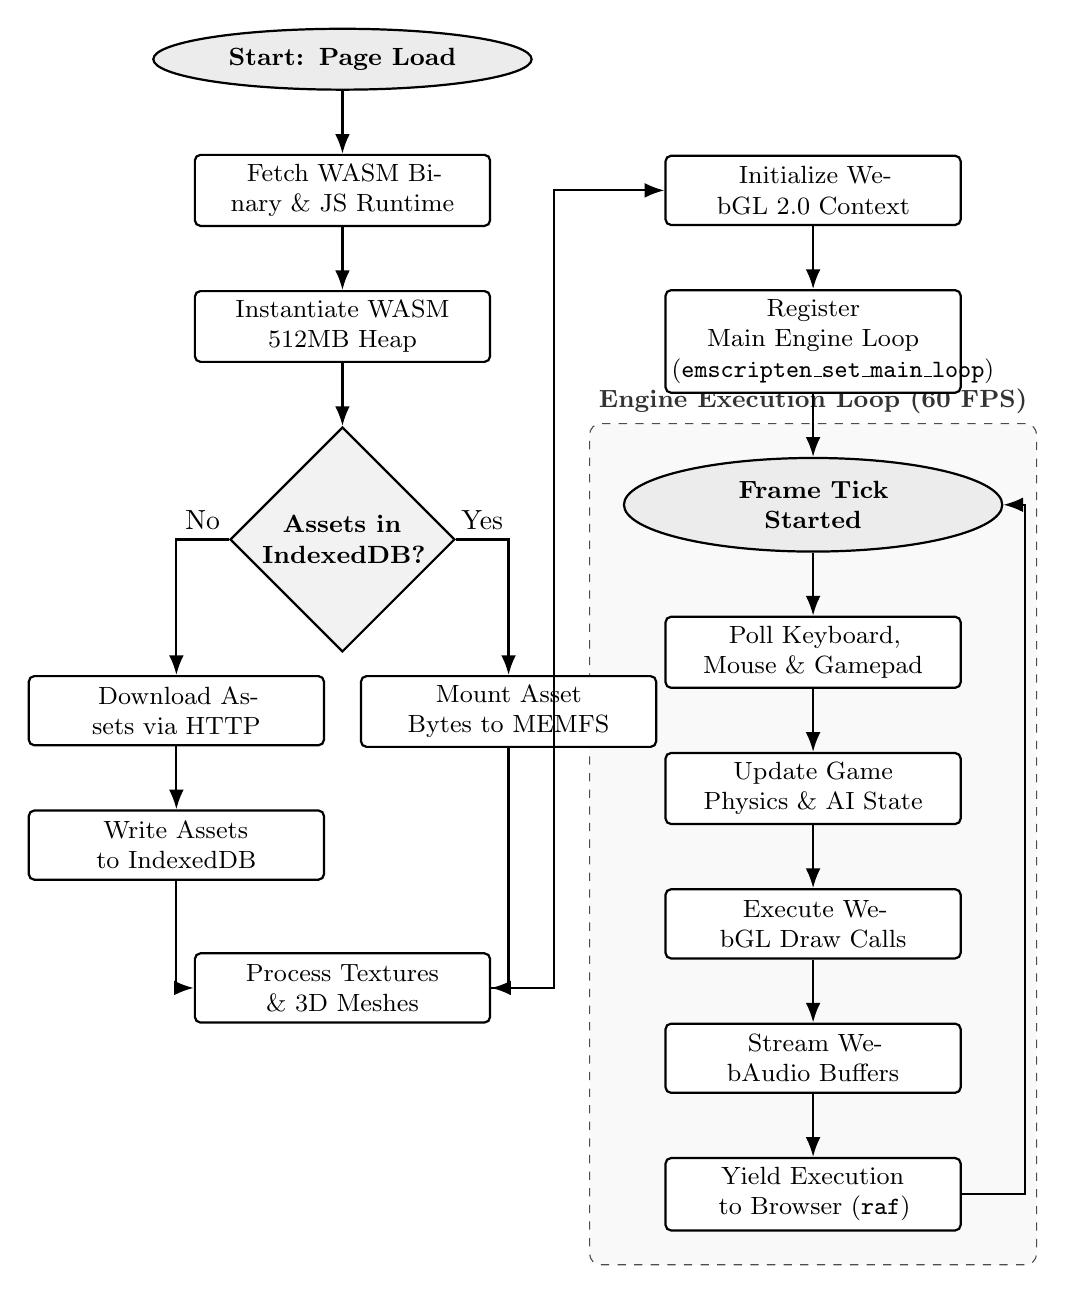
\begin{tikzpicture}[
    node distance=1.2cm and 1.8cm,
    auto,
    startstop/.style={ellipse, draw=black, thick, fill=gray!15, text width=9em, text centered, minimum height=2.2em, font=\small\bfseries},
    process/.style={rectangle, draw=black, thick, fill=white, text width=10em, text centered, rounded corners=2pt, minimum height=2.5em, font=\small},
    decision/.style={diamond, draw=black, thick, fill=gray!10, text width=6em, text centered, inner sep=1pt, font=\small\bfseries},
    loopbox/.style={rectangle, draw=black!70, dashed, fill=gray!5, inner sep=12pt, rounded corners=4pt},
    line/.style={draw=black, -{Latex[length=2.5mm]}, thick}
]

    % --- COLUMN 1: Bootstrapping & Asset Resolution ---
    \node [startstop] (start) {Start: Page Load};
    \node [process, below=0.8cm of start] (fetch) {Fetch WASM Binary \& JS Runtime};
    \node [process, below=0.8cm of fetch] (memory) {Instantiate WASM 512MB Heap};
    \node [decision, below=0.8cm of memory] (cache) {Assets in IndexedDB?};
    
    \node [process, below left=1.0cm and -0.5cm of cache] (http) {Download Assets via HTTP};
    \node [process, below=0.8cm of http] (idb) {Write Assets to IndexedDB};
    \node [process, below right=1.0cm and -0.5cm of cache] (load) {Mount Asset Bytes to MEMFS};

    \node [process, below=3.8cm of cache] (prep) {Process Textures \& 3D Meshes};

    % --- COLUMN 2: Subsystem Initialization & Runtime Main Loop ---
    \node [process, right=2.2cm of fetch] (webgl) {Initialize WebGL 2.0 Context};
    \node [process, below=0.8cm of webgl] (hook) {Register Main Engine Loop (\texttt{emscripten\_set\_main\_loop})};

    \node [startstop, below=0.8cm of hook] (tick) {Frame Tick Started};
    \node [process, below=0.8cm of tick] (input) {Poll Keyboard, Mouse \& Gamepad};
    \node [process, below=0.8cm of input] (physics) {Update Game Physics \& AI State};
    \node [process, below=0.8cm of physics] (draw) {Execute WebGL Draw Calls};
    \node [process, below=0.8cm of draw] (audio) {Stream WebAudio Buffers};
    \node [process, below=0.8cm of audio] (yield) {Yield Execution to Browser (\texttt{raf})};

    \begin{scope}[on background layer]
        \node [loopbox, fit=(tick) (input) (physics) (draw) (audio) (yield), label={[font=\small\bfseries\color{black!80}]above:Engine Execution Loop (60 FPS)}] (loop_frame) {};
    \end{scope}

    % --- PATH CONNECTIONS ---
    \path [line] (start) -- (fetch);
    \path [line] (fetch) -- (memory);
    \path [line] (memory) -- (cache);
    \path [line] (cache) -| node [near start, above] {No} (http);
    \path [line] (http) -- (idb);
    \path [line] (cache) -| node [near start, above] {Yes} (load);
    \path [line] (idb) |- (prep);
    \path [line] (load) |- (prep);

    \path [line] (prep.east) -- ++(0.8,0) |- (webgl.west);
    \path [line] (webgl) -- (hook);
    \path [line] (hook) -- (tick);

    \path [line] (tick) -- (input);
    \path [line] (input) -- (physics);
    \path [line] (physics) -- (draw);
    \path [line] (draw) -- (audio);
    \path [line] (audio) -- (yield);

    \path [line] (yield.east) -- ++(0.8,0) |- (tick.east);

\end{tikzpicture}
}
\caption{System Activity Diagram showing engine bootstrapping, virtual asset mounting, and browser-yielded rendering main loop.}
\label{fig:activity}
\end{figure}

\begin{figure}[H]
    \centering
    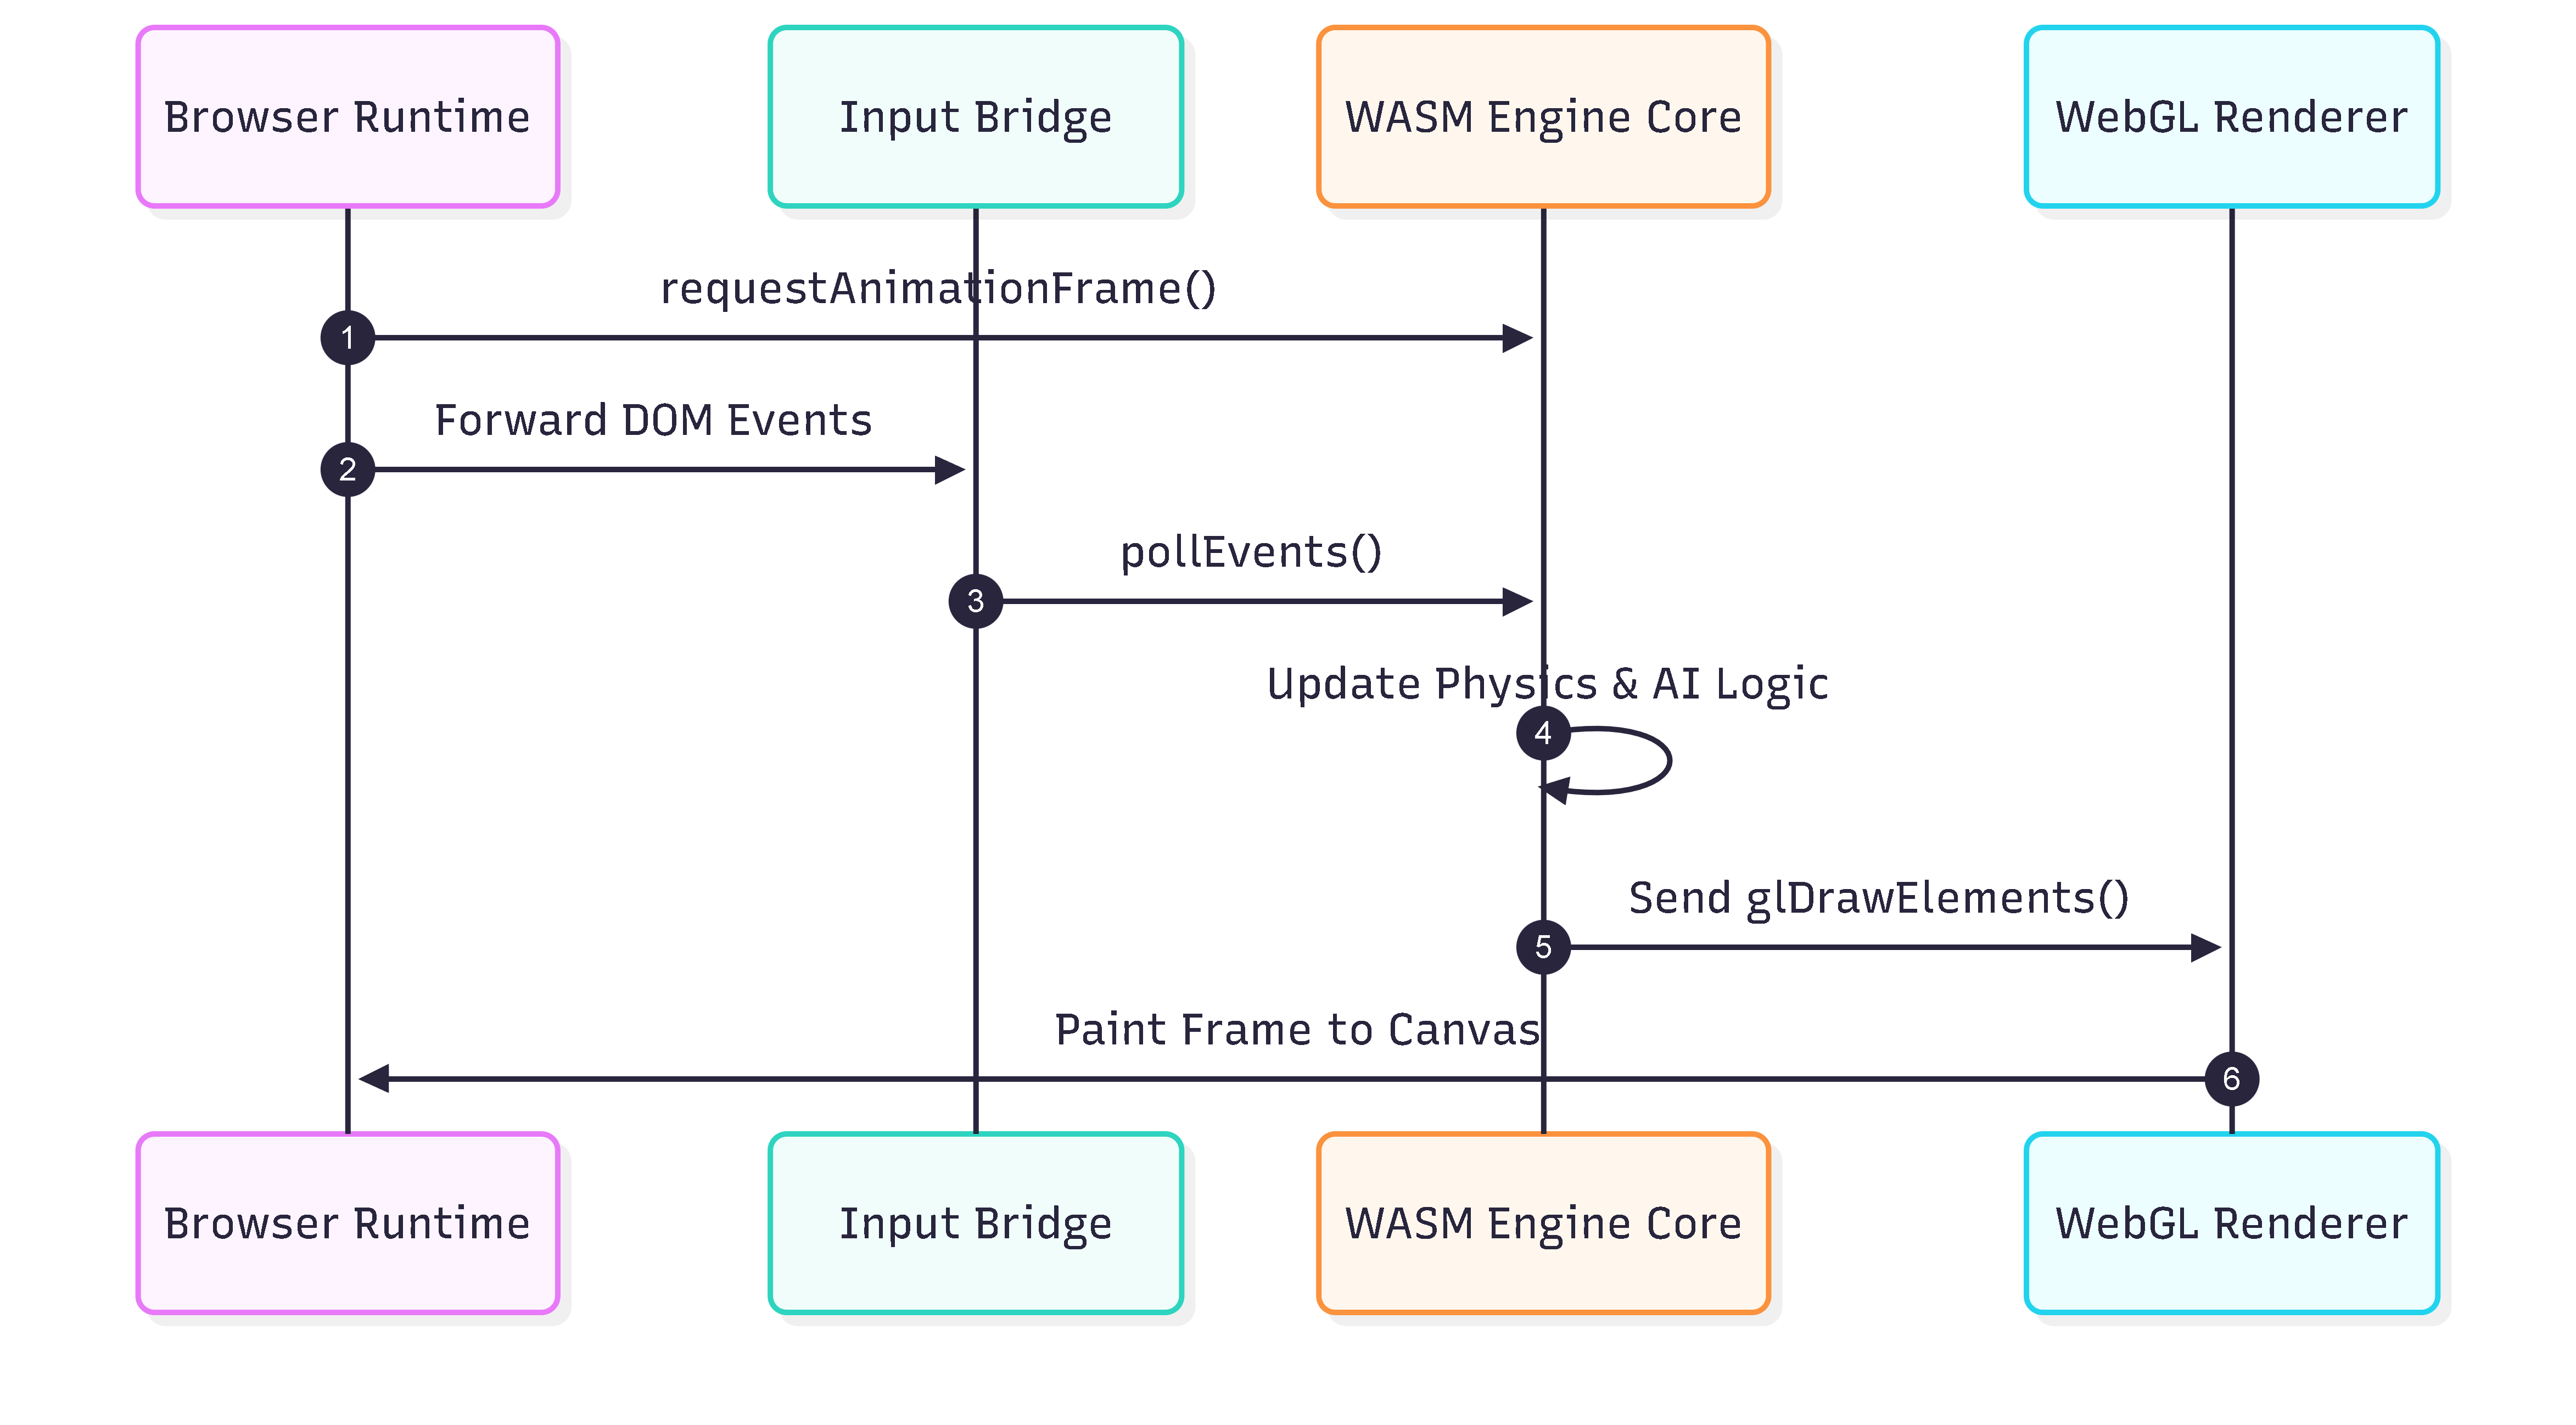
\includegraphics[width=0.85\textwidth]{sequence_diagram.png}
    \caption{Sequence Diagram showing WebGL context initialization and WASM call stack.}
    \label{fig:sequence}
\end{figure}

\begin{figure}[H]
    \centering
    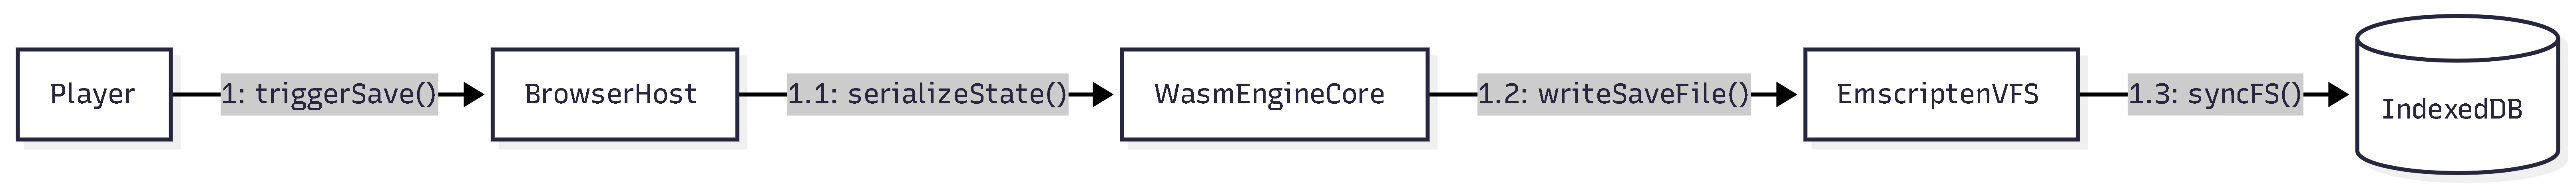
\includegraphics[width=0.8\textwidth]{collaboration_diagram.png}
    \caption{Collaboration Diagram detailing object interaction paths.}
    \label{fig:collaboration}
\end{figure}

\section{Testing & Preliminary Results}

\subsection{Evaluation Methodology}
Performance tests were conducted on Google Chrome (v120+) using a 1080p display context. Diagnostics focused on load times, WASM memory footprint, rendering frame rates, and input responsiveness.

\subsection{Observed Data}
\begin{itemize}
    \item \textbf{Compilation Output Size:} Final compressed build output consists of a $12\,\text{MB}$ JS/WASM package (excluding game assets).
    \item \textbf{Render Performance:} Stable execution at $30\text{--}60\,\text{FPS}$ during static menu interaction and localized indoor rendering tests.
    \item \textbf{Memory Allocation:} Average operational memory draw settled at approximately $310\,\text{MB}$ of WASM linear memory heap.
\end{itemize}

\section{Limitations \& Known Issues}

\begin{itemize}
    \item \textbf{Asset Loading Latency:} Downloading large monolithic asset files (\texttt{GTA3.IMG}, $\sim 500\,\text{MB}$) over HTTP creates a significant startup delay.
    \item \textbf{Single-Threaded Constraints:} Audio processing and asset streaming share the main browser thread, causing minor audio micro-stutters during heavy scene transitions.
\end{itemize}

\section{Future Work \& Roadmap}

\begin{enumerate}
    \item \textbf{Asset Chunking \& Caching:} Implement HTTP Range Requests and IndexedDB client-side caching to load game models on-demand.
    \item \textbf{Multithreading Integration:} Migrate physics computations and audio decoding to Web Workers using WebAssembly pthreads (\texttt{SharedArrayBuffer}).
    \item \textbf{Touch Control Layer:} Add virtual joystick overlays for mobile browser compatibility.
\end{enumerate}
\begin{figure}[H]
\centering
\resizebox{\textwidth}{!}{%
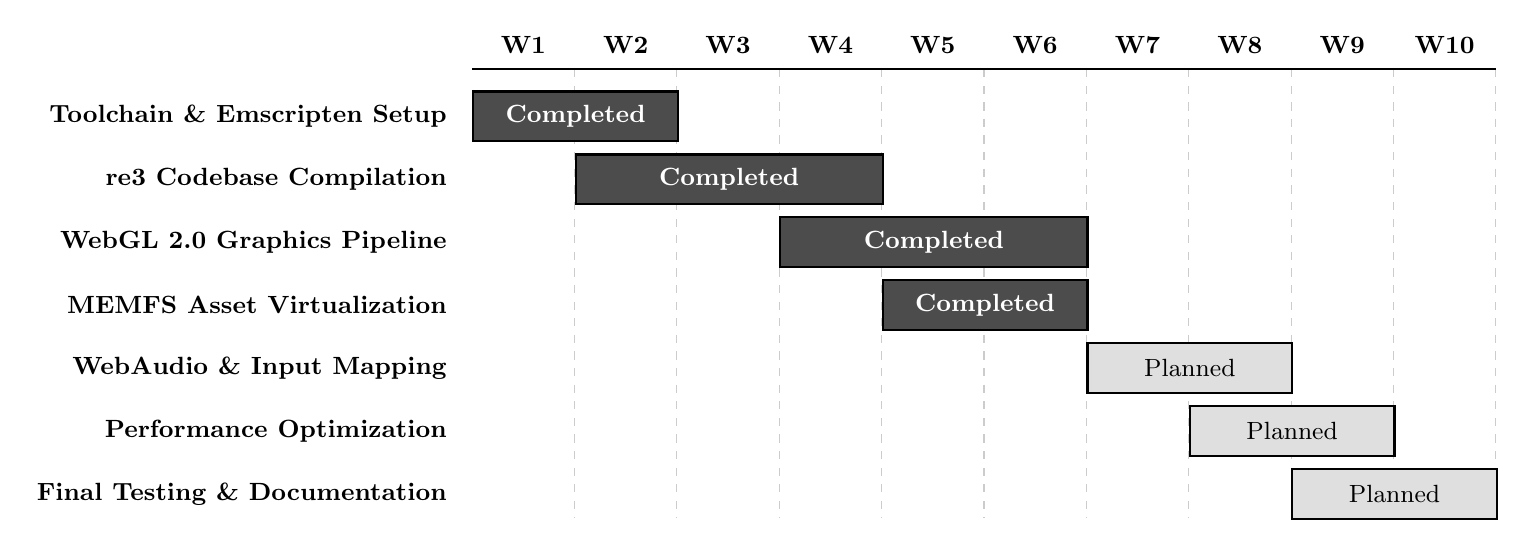
\begin{tikzpicture}[
    task/.style={rectangle, draw=black, thick, fill=gray!25, minimum height=1.8em, align=left, font=\small},
    completed/.style={rectangle, draw=black, thick, fill=black!70, text=white, minimum height=1.8em, align=left, font=\small\bfseries},
    gridline/.style={draw=black!20, dashed},
    labelnode/.style={anchor=east, font=\small\bfseries, align=right}
]

    % --- Grid Timeline Header (Weeks 1 to 10) ---
    \foreach \w in {1,...,10} {
        \node[font=\small\bfseries] at (\w*1.3 - 0.65, 0.5) {W\w};
        \draw[gridline] (\w*1.3, 0.2) -- (\w*1.3, -5.5);
    }
    \draw[thick] (0, 0.2) -- (13, 0.2);

    % --- Task Labels ---
    \node[labelnode] at (-0.2, -0.4) {Toolchain \& Emscripten Setup};
    \node[labelnode] at (-0.2, -1.2) {re3 Codebase Compilation};
    \node[labelnode] at (-0.2, -2.0) {WebGL 2.0 Graphics Pipeline};
    \node[labelnode] at (-0.2, -2.8) {MEMFS Asset Virtualization};
    \node[labelnode] at (-0.2, -3.6) {WebAudio \& Input Mapping};
    \node[labelnode] at (-0.2, -4.4) {Performance Optimization};
    \node[labelnode] at (-0.2, -5.2) {Final Testing \& Documentation};

    % --- Task Bars (Completed vs Planned) ---
    % Completed Tasks
    \node[completed, anchor=west, minimum width=2.6cm] at (0, -0.4) {Completed};
    \node[completed, anchor=west, minimum width=3.9cm] at (1.3, -1.2) {Completed};
    \node[completed, anchor=west, minimum width=3.9cm] at (3.9, -2.0) {Completed};
    \node[completed, anchor=west, minimum width=2.6cm] at (5.2, -2.8) {Completed};

    % Planned Future Tasks
    \node[task, anchor=west, minimum width=2.6cm] at (7.8, -3.6) {Planned};
    \node[task, anchor=west, minimum width=2.6cm] at (9.1, -4.4) {Planned};
    \node[task, anchor=west, minimum width=2.6cm] at (10.4, -5.2) {Planned};

\end{tikzpicture}
}
\caption{Project Gantt Chart mapping completed prototype milestones and future development phases.}
\label{fig:gantt}
\end{figure}
\end{document}
